
% Formatka dla raportów projektowych dla Koła Naukowego KoNaR 
% Autor: Bartosz Kolasa
% Edycja: Michał Swoboda
% Edycja2: Bartłomiej Kurosz
% Treść: Bartłomiej Kurosz

%-------------------------------------
% Definicja klasy dokumentu
\documentclass[12pt,a4paper]{article}

%------------------------------------
% 			Pakiety
\usepackage[utf8x]{inputenc}
\usepackage{ucs}
\usepackage[MeX]{polski}
\usepackage{fancyhdr}
\usepackage{amsmath}
\usepackage{amsfonts}
\usepackage{amssymb}
\usepackage{subfig}
\usepackage[hidelinks]{hyperref}
\usepackage{graphicx}
\pagestyle{fancy}

%---------------------------------------
% 		Dodanie strony tytulowej do dokumentu

\renewcommand{\maketitle}{\begin{titlepage}

\begin{center}

\includegraphics[scale=1]{figures/logo.png}
\vspace*{0.5cm}
\noindent \rule{\linewidth}{0.4mm}
\LARGE \textsc{Robot mobilny klasy Line Follower}\\
\LARGE \textsc{Maverick}
\vspace*{0.5cm}
\rule{\linewidth}{0.4mm}
\vspace*{1.5cm}

\large
\textsc{Łukasz Michalczak} \\
\textsc{Anna Postawka}\\

\vspace*{4cm}
\textsc{Koło Naukowe Robotyków KoNaR }\\
\textsc{\url{www.konar.pwr.edu.pl}}\\
\textsc{6 stycznia 2016}\\
\end{center}
\end{titlepage}
\newpage
} % W tym pliku należy w odpowiednim miejscu wpisać członków zespołu

%-----------------------------------------
% 		Poczatek dokumentu
\begin{document}
\maketitle % Komenda maktitle dodaje stronę tytułową do dokumentu głównego
\tableofcontents % Komenda tableofcontents dodaje spis treści do dokumentu głównego
\newpage % Komenda newpage przechodzi do nowej strony w dokumencie.

%------------------------------------------
%			Streszczenie (MOŻNA POMINĄĆ)
%\begin{abstract}
% Tu należy zamieścić streszczenie projektu.
%\end{abstract}

%------------------------------------------
%				Dokument wlasciwy
\section{Wstęp}
Maverick to robot klasy Line Follower Light. Został stworzony w ramach warsztatów robotycznych organizowanych w 2015 r. przez koło naukowe \mbox{KoNaR} działające na Politechnice Wrocławskiej. Celem było wystartowanie w zawodach Robotic Arena 2015. Opiekunem projektu został Bartek Kurosz. Był on nieocenioną pomocą i znacznie przyczynił się do sukcesu tej konstrukcji.

Głównym założeniem było po prostu stworzenie działającej maszyny, jako że był to pierwszy robot jego autorów. Ale na początku pracy, podczas intensywnego zbierania inspiracji i informacji na temat tego typu konstrukcji wykrystalizowała się wizja, aby stworzyć robota jak najlżejszego, bez zbędnych elementów, ale takiego, który pozwalałby na osiąganie dobrych wyników i konkurowanie z najlepszymi.

Dokument ten przedstawia poszczególne elementy budowy Mavericka oraz opisuje koncepcję zaimplementowanego programu.


\section{Maverick}

\begin{figure}[tp]
\centering
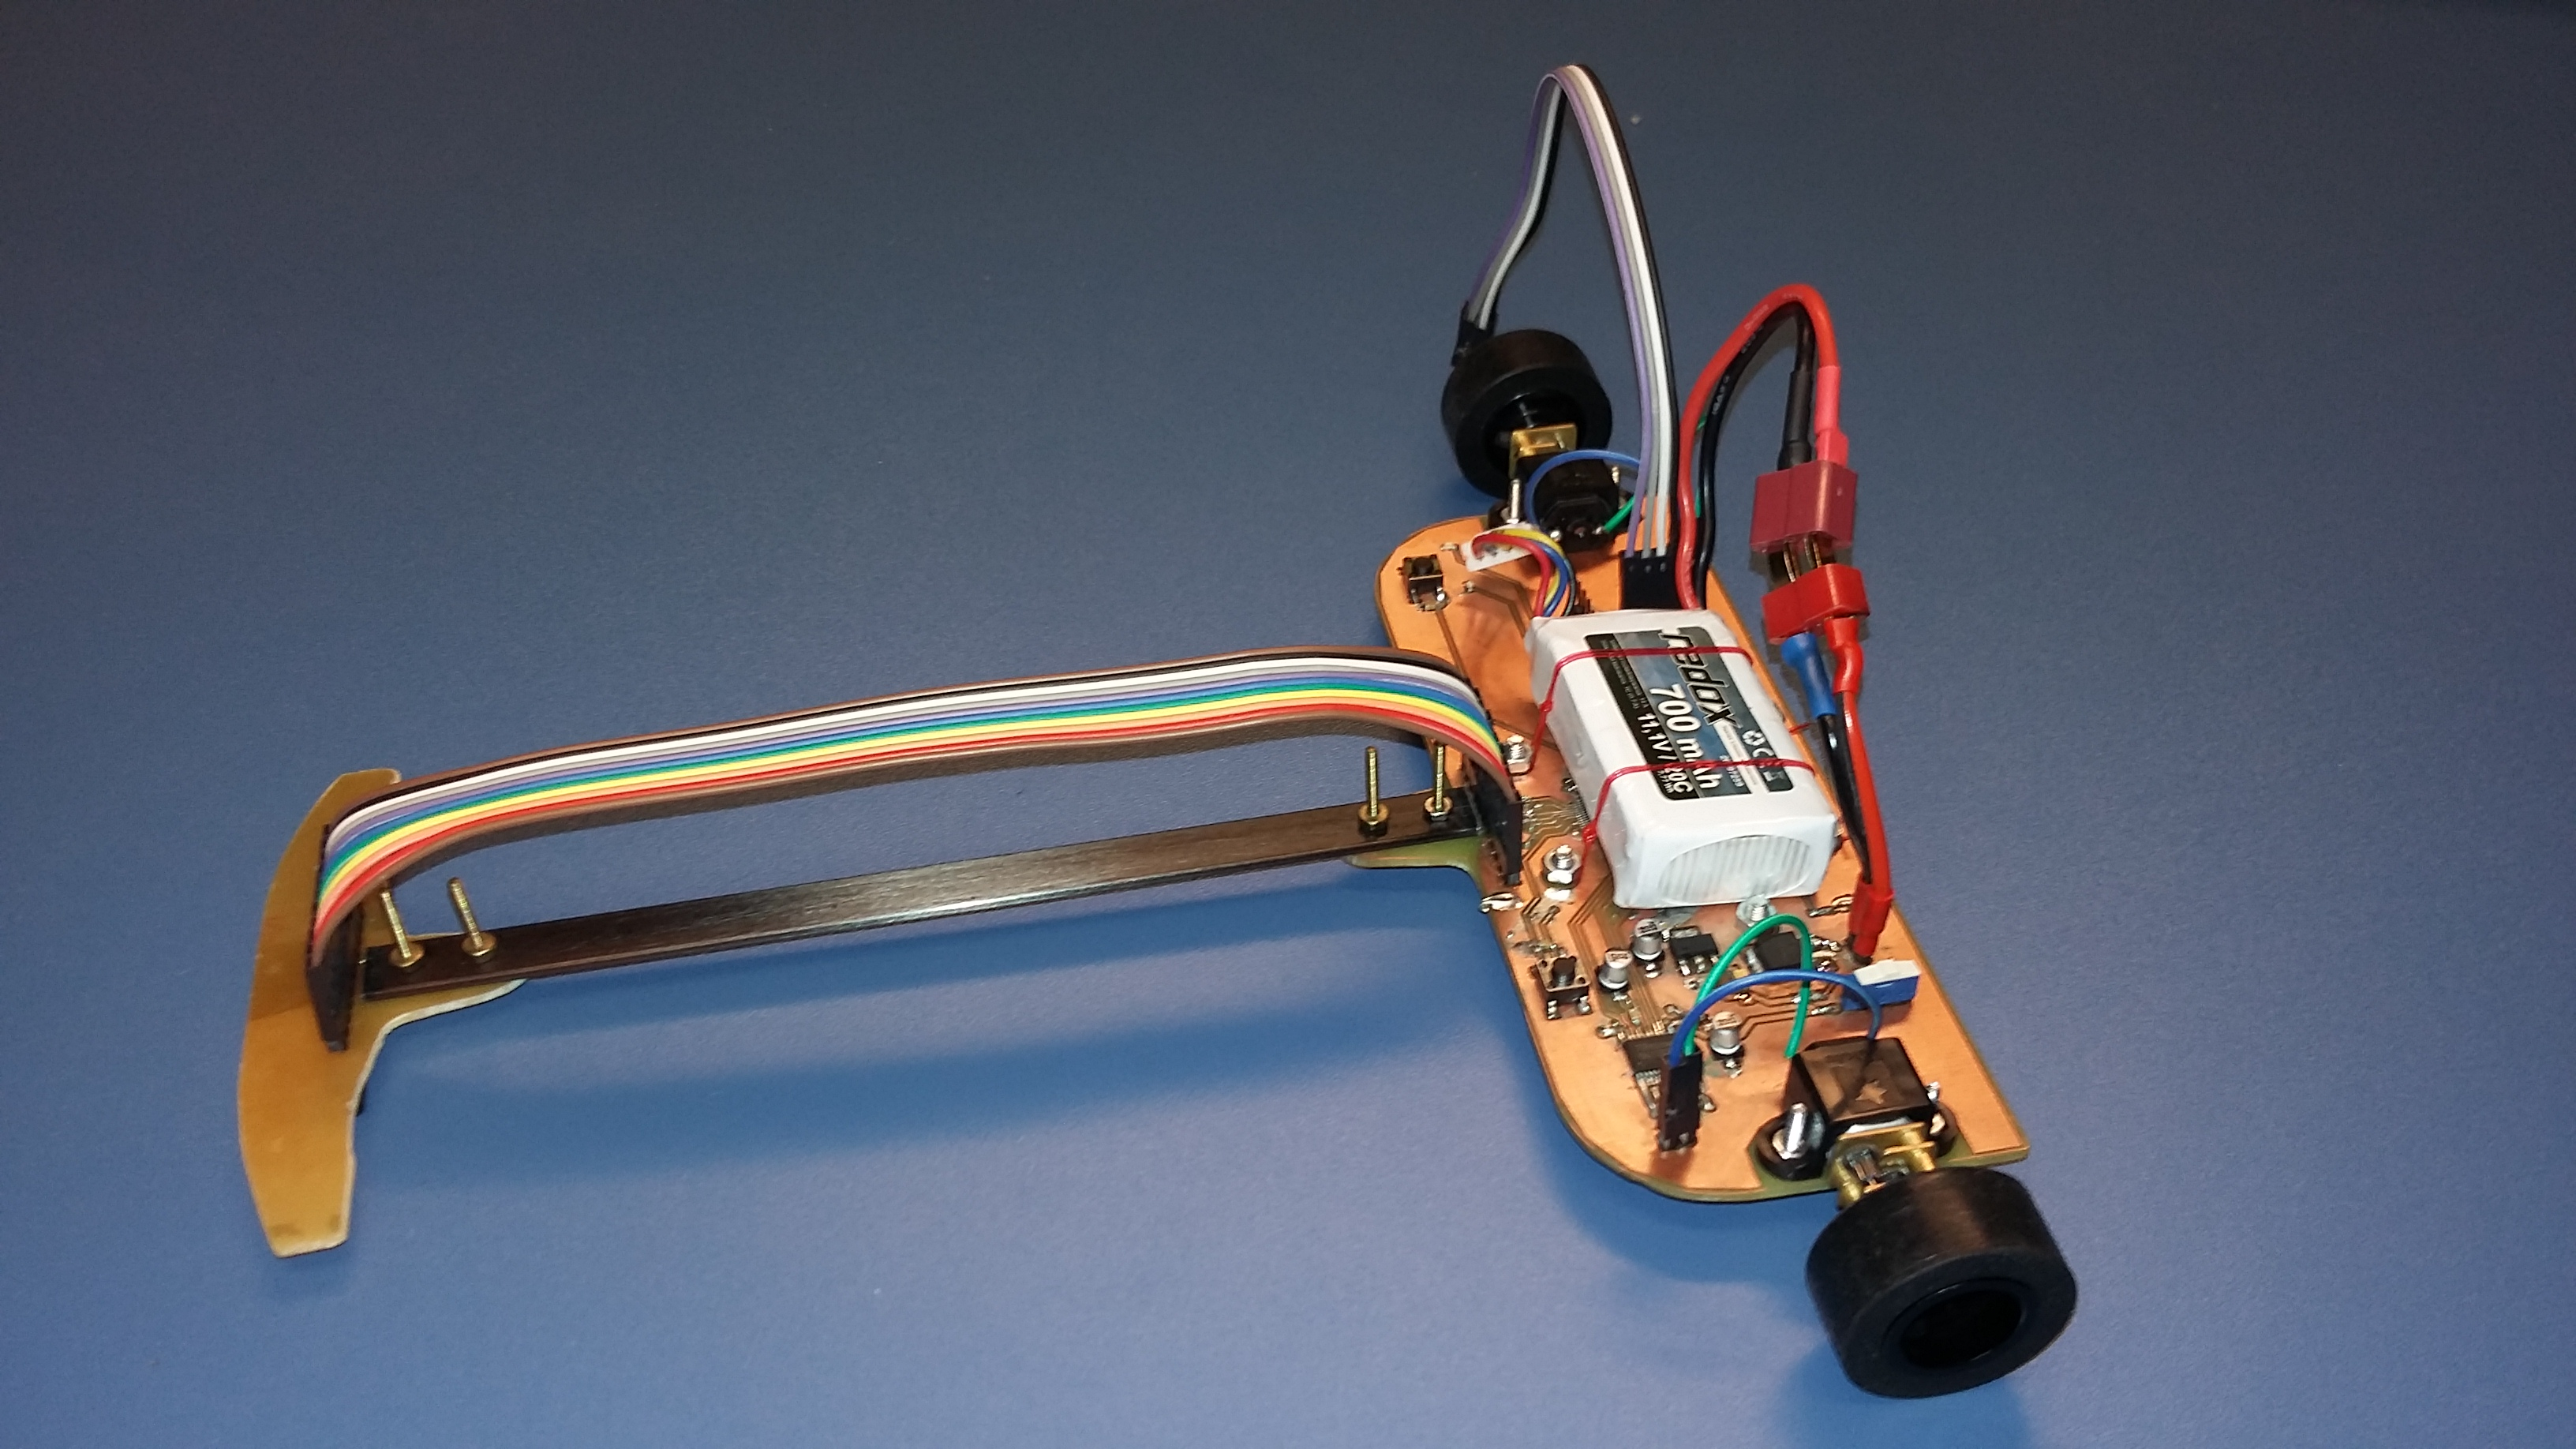
\includegraphics[width=0.9\textwidth]{figures/6.jpg}
\caption{Robot mobilny Maverick \label{fig:mav}}
\end{figure}

\subsection{Mechanika}
Podstawą konstrukcji robota (rysunek \ref{fig:mav}) są dwie płytki PCB. 
Zostały one połączone listewką węglową. Na przedniej płytce znajdują się tylko czujniki, na tylnej cała reszta elektroniki. Silniki i akumulator są przymocowane bezpośrednio do płytki.

Taka konstrukcja ma wiele zalet. Przede wszystkim jest lekka, bo nie trzeba wprowadzać dodatkowych elementów stanowiących podwozie czy ramę pojazdu. Dodatkowo można zmieniać odległość płytek od siebie. Problemem mogłoby być to, że bezpośrednie przykręcenie układu napędowego do płytki PCB może narażać elektronikę na potencjalnie szkodliwe wstrząsy, ale jak na razie nie zostały zauważone żadne negatywne skutki takiej budowy.


\subsubsection{Listewka węglowa}
Zostały przetestowane dwie długości listewki: 12 cm i 16 cm. Dłuższa sprawdziła się lepiej. W przyszłości warto by było przetestować jeszcze inne długości (max. 26 cm, aby robot mieścił się na kartce A4), aby dobrać najlepszą optymalną dla tej konstukcji. Można by też spróbować zastosować lżejszy materiał.


\subsubsection{Koła}
Zamontowane zostały koła Solarbotics RW2i razem z oponami. Zapewniły one wystarczającą przyczepność.

\subsubsection{Akumulator}
Akumulator został umieszczony na tylnej osi, aby dociążyć koła i zwiększyć przyczepność. Został przymocowany gumkami zawiązanymi do śrubek przykręconych do płytki PCB. Na przyszłość warto by pomyśleć nad innym mocowaniem - po pierwsze śrubki są niepotrzebnym ciężarem, po drugie aktualnie nie ma możliwości przesunięcia akumulatora, a jest to jeden z cięższych elementów konstrukcji i znacznie zmienia on wyważenie robota, co może wpływać na osiągi.

Aktualnie akumulator leży na podwyższeniu, co ma uchronić delikatne elementy znajdujące się pod nim od uszkodzenia mechanicznego. Nie jest to najlepsze rozwiązanie - dla zwiększenia przyczepności lepiej byłoby umieścić akumulator jak najniżej. Jeśli zostałaby wykonana nowsza wersja płytki, trzeba by było najpierw eksperymentalnie wyznaczyć najlepsze ustawienie akumulatora względem osi kół, po czym przeprojektować płytkę tak, aby przesunąć elementy spod akumulatora w inne miejsce i może nawet wyciąć dziurę w płytce, aby ten ciężar znalazł się jak najbliżej podłoża.



\subsection{Elektronika}
Elektronika została zaprojektowana w programie KiCad. Jest to oprogramowanie typu open source przeznaczone do edycji schematów oraz obwodów drukowanych. 

Płytki były przygotowywane samodzielnie, więc w projekcie unikano umiejscawiania elementów czy ścieżek zbyt blisko siebie oraz w pobliżu krawędzi. Ograniczono również ilość przelotek, gdyż ich wykonanie jest czasochłonne i wymaga dużej precyzji. Użyto głównie elementów powierzchniowo montowanych (ang. SMD, Surface Mounted Devices). Zajmują one mniej miejsca i nie potrzebują dodatkowych otworów. Zastosowano technikę fotochemiczną.

Ścieżki, przez które prąd z akumulatora płynie bezpośrednio, są szersze (mają 32 milsy). Dla najważniejszych elementów, takich jak mikrokontroler czy sterownik silników, poprowadzono osobne ścieżki zasilania. Zakłócenia są filtrowane za pomocą kondensatorów.


%Tutaj warto zawrzeć informacje o programie w którym ją tworzyliśmy, o tym jak była projektowana płytka ze względu na metodę tworzenia (czyli robiliśmy fototransferem, więc nie mogliśmy robić ultra cienkich ścieżek, minimalizowaliśmy ilość przelotek bo przecież kto to będzie tyle wiercił i lutował, staraliśmy się dawać większe pady do elementów przewlekanych i przelotek itp.)
\subsubsection{Zasilanie}
Do zasilania użyto akumulatora Li-pol. Podzespoły pracują pod napięciem 3,3V. Wyjątkiem są silniki, do których prąd dostarczany jest bezpośrednio z zasilacza. Do uzyskania pożądanego napięcia użyto stabilizatora LM1117S 3,3V/1A. Zastosowano zabezpieczenie przed odwrotną polaryzacją układu w postaci tranzystora typu P. Wykorzystano suwakowy przełącznik zasilania. Poprawne zasilanie sygnalizowane jest poprzez diodę LED. 
Na rysunku \ref{fig:zasilanie} przedstawiono schemat zasilania.
%
\begin{figure}[tp]
\centering
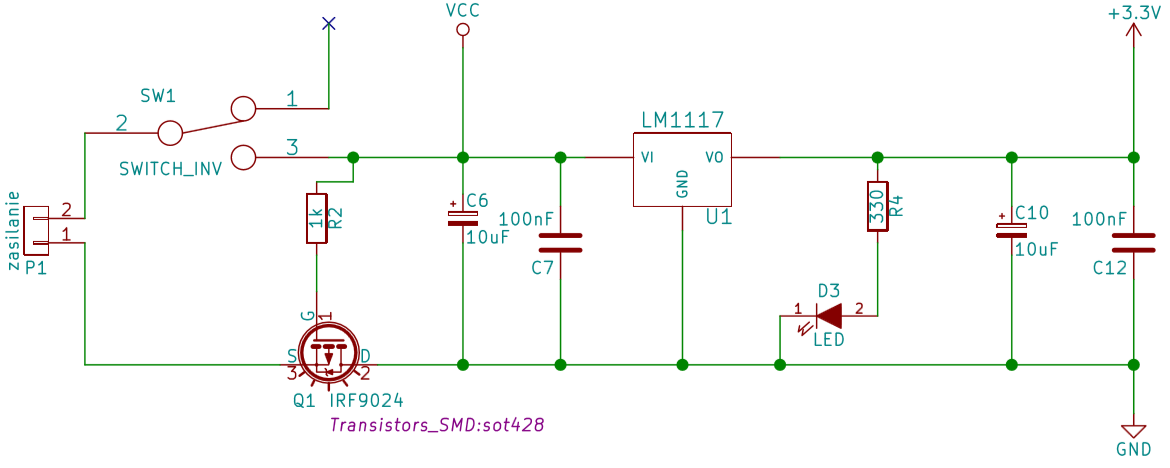
\includegraphics[width=1\textwidth]{figures/zasilanie.png}
\caption{Zasilanie \label{fig:zasilanie}}
\end{figure}


\subsubsection{Mikrokontroler}
Użyto mikrokontrolera STM32F100C4T6B.

Specyfikacja: 
\begin{itemize}
\item Maksymalne taktowanie: 24MHz
\item Napięcie pracy: 2,0 - 3,6V
\item Pamięć Flash: 16kB
\item Pamięć RAM: 4kB
\item Przetwornik ADC: 10 kanałowy, 12 bitowy
\item Interfejs: I2C, SPI, USART
\item Liczba timerów: 6 (pięć 16 bitowych)
\item Liczba wejść/wyjść: 37
\item Obudowa: LQFP48
\end{itemize}

Debugowanie ułatwiają dwie diody LED (rys. \ref{fig:komunikacja}).

Początkowo użyto mikrokontrolera STM32F100C8T6B, jednak uległ on uszkodzeniu. Powyższego mikrokontrolera użyto jako zamiennika, gdyż poprzedni był już niedostępny. Należało połączyć wyprowadzenia generujące sygnał PWM ze sterownikiem silników za pomocą izolowanych przewodów, ponieważ występowała niezgodność timerów w stosunku do pierwotnego układu.

Schemat mikrokontrolera (rys.\ref{fig:uc}) oraz jego zasilanie (rys.\ref{fig:uc_sup}).
\begin{figure}[tp]
\centering
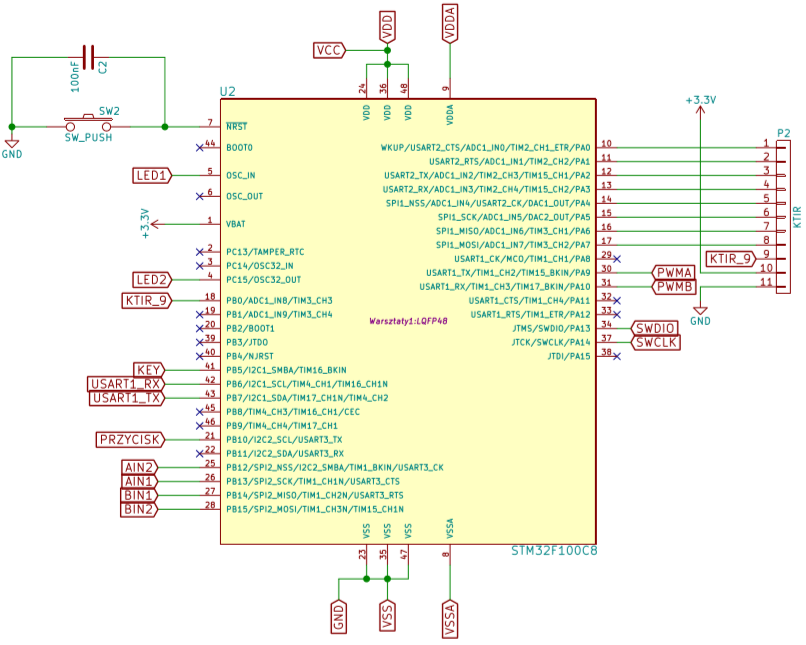
\includegraphics[width=1\textwidth]{figures/uc.png}
\caption{Mikrokontroler \label{fig:uc}}
\end{figure}
\begin{figure}[tp]
\centering
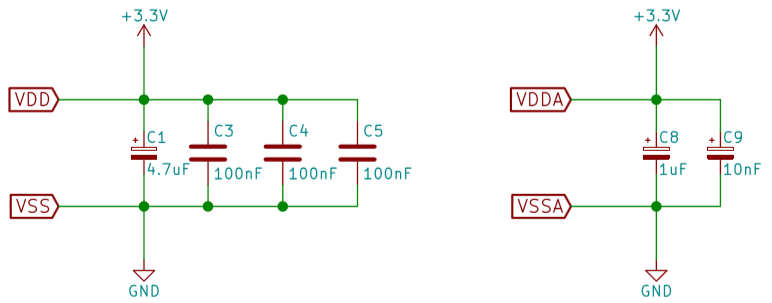
\includegraphics[width=0.7\textwidth]{figures/uc_sup.png}
\caption{Zasilanie mikrokontrolera \label{fig:uc_sup}}
\end{figure}


\subsubsection{Czujniki}
Do wykrywania czarnej linii zastosowano 9 czujników optycznych KTIR0711S.

Odczyt wykonywany jest z użyciem przetwornika ADC mikrokontrolera.

Specyfikacja:
\begin{itemize}
\item Napięcie diody: 5V
\item Maksymalny prąd diody: 50mA
\item Maksymalne napięcie kolektor-emiter: 30V
\item Maksymalny prąd kolektora: 20mA
\item Odległość pomiaru: max 0,5cm
\end{itemize}

Na rysunku \ref{fig:ktir} przedstawiono schemat podłączenia czujnika optycznego.
%
\begin{figure}[tp]
\centering
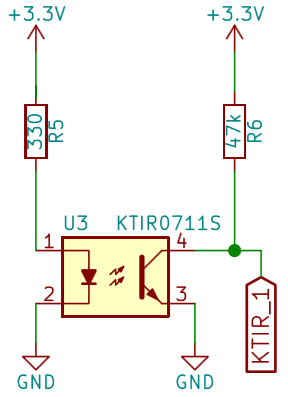
\includegraphics[width=0.3\textwidth]{figures/ktir.png}
\caption{Czujnik optyczny \label{fig:ktir}}
\end{figure}


\subsubsection{Sterowanie silnikami}
Do sterowania silnikami użyto podwójnego mostka H TB6612.

Układ pozwala na proste i niezależne sterowanie dwoma silnikami DC.

Specyfikacja:
\begin{itemize}
\item Napięcie logika: 2,7V - 5,5V
\item Napięcie silnik: 4,5V - 13,5V
\item Ciągły prąd wyjścia na kanał: 1,2A
\item Chwilowy prąd wyjścia na kanał: 3,2A
\item Obudowa: SSOP24-szeroki - 8,3x7,6x1,6mm
\end{itemize}

Na rysunku \ref{fig:h} przedstawiono schemat podłączenia sterownika silników.
%
\begin{figure}[tp]
\centering
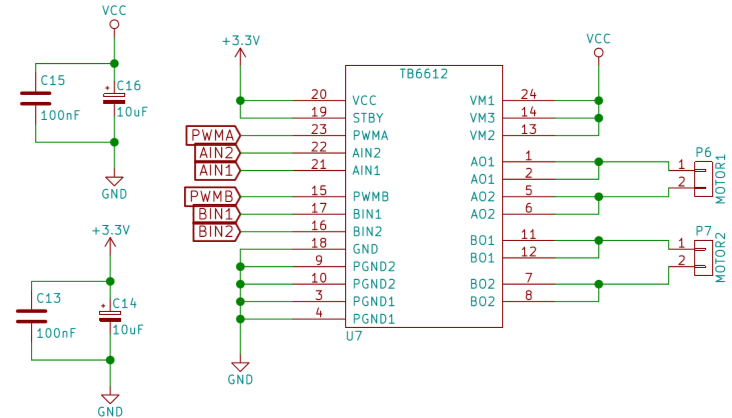
\includegraphics[width=1\textwidth]{figures/h_and_sup.png}
\caption{Sterownik silników \label{fig:h}}
\end{figure}


\subsubsection{Interfejs komunikacyjny}
Zastosowano przycisk generujący przerwanie oraz drugi, wywołujący reset mikrokontrolera.

Programowanie dokonywane jest poprzez czteropinowe złącze SWD programatora. Wyprowadzono również złącze na moduł bluetooth. Zamontowano diodę sygnalizującą poprawne zasilanie oraz dwie diody programowalne.  
Ostatecznie moduł bluetooth nie został użyty ze względu na brak czasu oraz niezgodność z wyprowadzeniami złącza.

Schematy interfejsów komunikacyjnych przedstawia rysunek \ref{fig:komunikacja}.
%
\begin{figure}[tp]
\centering

    \subfloat[Przycisk\label{subfig:Przycisk}]{%
      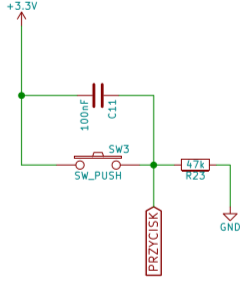
\includegraphics[width=0.3\textwidth]{figures/button.png}
    } %Miedzy tymi obrazkami nie ma przerwy, wiec beda zestawione poziomo
    \hspace{0.4cm}
    \subfloat[Diody\label{subfig:Diody}]{%
      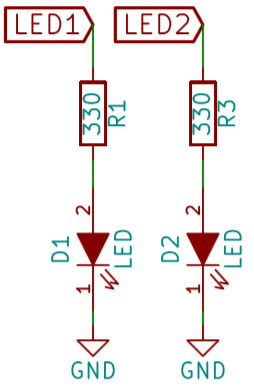
\includegraphics[width=0.23\textwidth]{figures/led.png}    
    }%Ponizej jest przerwa, wiec nastapi przejscie do nowej linii


    \subfloat[Bluetooth\label{subfig:Bluetooth}]{%
      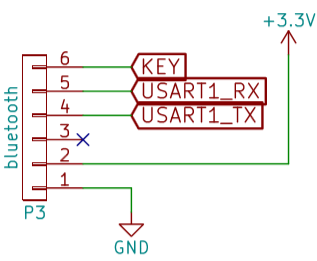
\includegraphics[width=0.3\textwidth]{figures/bt.png}
    }
    \hspace{0.4cm}
	\subfloat[Programator\label{subfig:Programator}]{%
      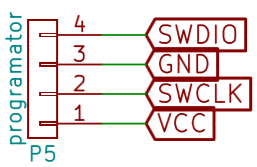
\includegraphics[width=0.3\textwidth]{figures/programator.png}
    } 
    \caption{Interfejsy komunikacyjne}
    \label{fig:komunikacja}
  \end{figure}%


\subsection{Program}
Program napisany jest w języku C. Korzystano z darmowego, zintegrowanego środowiska programistycznego dla mirokontrolerów STM32 i związanych z nimi płytek.

STM32CubeMX jest graficznym narzędziem konfiguracyjnym, pozwalającym na generowanie gotowego kodu w języku C dla wybranego mikrokontrolera. 
System Workbench for STM32 to środowisko programistyczne oparte na oprogramowaniu Eclipse, które wspiera pełną gamę mikrokontrolerów STM32. Pozwala na programowanie i debugowanie urządzenia.

Pomocne okazały się również darmowe programy STM32 ST-LINK Utility, jako alternatywne narzędzie do programowania i łączenia się z mikrokontrolerem oraz 
STMStudio, pozwalający na monitorowanie wartości zmiennych podczas pracy robota, który w szczególności użyty został do testu czujników linii.


\subsubsection{Konfiguracja peryferii}
Do wykrywania czarnej linii wykorzystano przetwornik ADC. Skonfigurowany został do pracy w trybie DMA (Direct Memory Access, z ang. bezpośredni dostęp do pamięci). Technologia ta pozwala na transfer danych pomiędzy pamięcią a peryferiami z pominięciem procesora. Wykorzystana została do zapisu odczytów z czujników optycznych. 

Sterowanie sinikami oparte zostało na generacji sygnału PWM przez timer. Prescaler ustawiono na wartość 23, a AutoReload Register na 999. Umożliwia to regulacje mocą silnika na przedziale [0;1000]. Jest to w wystarczająca rozdzielczość w zastosowaniu do line followera. Przy taktowaniu 24MHz częstotliwość przerwań wynosi 1000Hz.

Pętla algorytmu sterowania robotem jest wykonywana w przerwaniu timera z częstotliwością 100Hz. Długość przerw wpływa na efekt działania członu różniczkującego regulatora. 


\subsubsection{Algorytm sterowania}
Algorytm sterowania robota oparty jest o regulator PD (proporcjonalno-różniczkujący) wykonywany w przerwaniu timera z częstotliwością 100Hz. Odczyt z czujników, na podstawie którego obliczany jest uchyb regulacji, wykonywany jest w trybie DMA. Następnie na silnik podawana jest nowa wartość mocy z dostępnego przedziału wyznaczona poprzez regulator. 

Istotnym elementem algorytmu jest zapamiętywanie ostatniego błędu położenia względem linii. Wypadnięcie z trasy skutkuje zwiększonym uchybem. Zastosowano stopniowe rozpędzanie przy starcie, gdyż unosiła się przednia część robota.  


\section{Podsumowanie}

W dokumencie opisano proces budowy robota klasy Line Follower. Prace nad nim trwały od 8 listopada do 12 grudnia, czyli trochę ponad miesiąc. Cel został osiągnięty: udało się wystawić Mavericka na Robotic Arenie 2015. Podczas zawodów robot nie sprawiał żadnych problemów, więc można się było skupić na testowaniu różnych parametrów i ustawień. Maverick poradził sobie zadziwiająco dobrze - w klasie Line Follower Light uzyskał 6. miejsce, czyli niewiele brakowało, a wszedłby do finału.

%Przez miesiąc prac nad robotem nauczyliśmy się niesamowicie dużo i sprawiło nam to wielką frajdę. Chociaż czasem bywało ciężko (miesiąc to jednak niewiele czasu, żeby będąc totalnym laikiem stworzyć coś od podstaw), to na pewno było warto!

Podsumowując, robot przeszedł najważniejszą próbę i sprawdził się na zawodach. Okazał się dobrą konstrukcją, w której jednak nadal jest sporo rzeczy, które można ulepszyć. Przy dalszych pracach nad Maverickiem warto byłoby skupić sie na następujących kwestiach:
\begin{itemize}
\item Odchudzenie konstrukcji: wymiana listewki, zmiana sposobu mocowania akumulatora.
\item Zwiększenie przyczepności: lepsze wyważenie dzięki przeniesieniu akumulatora, odlanie własnych opon.
\item Zmniejszenie lub zlikwidowanie opóźnienia: prawdopodobnie dzięki lepszemu wyważeniu można by zniwelować podrywanie się przodu przy starcie.
\item Ulepszenie algorytmu.
\end{itemize}


\section{Materiały źródłowe}
Korzystano z wiedzy uzyskanej na warsztatach robotycznych oraz z wielu materiałów ogólnodostępnych w sieci. Najbardziej pomocna okazała się strona \url{www.forbot.pl} oraz KoNaRowe archiwum: \url{http://lirec.iiar.pwr.edu.pl/~konarch/download/linefollower/}

%\bibliographystyle{plunsrt}
%\bibliography{mybib}
\clearpage

\begin{figure}[tp]
\centering

    \subfloat[Widok z góry\label{subfig:m2}]{%
      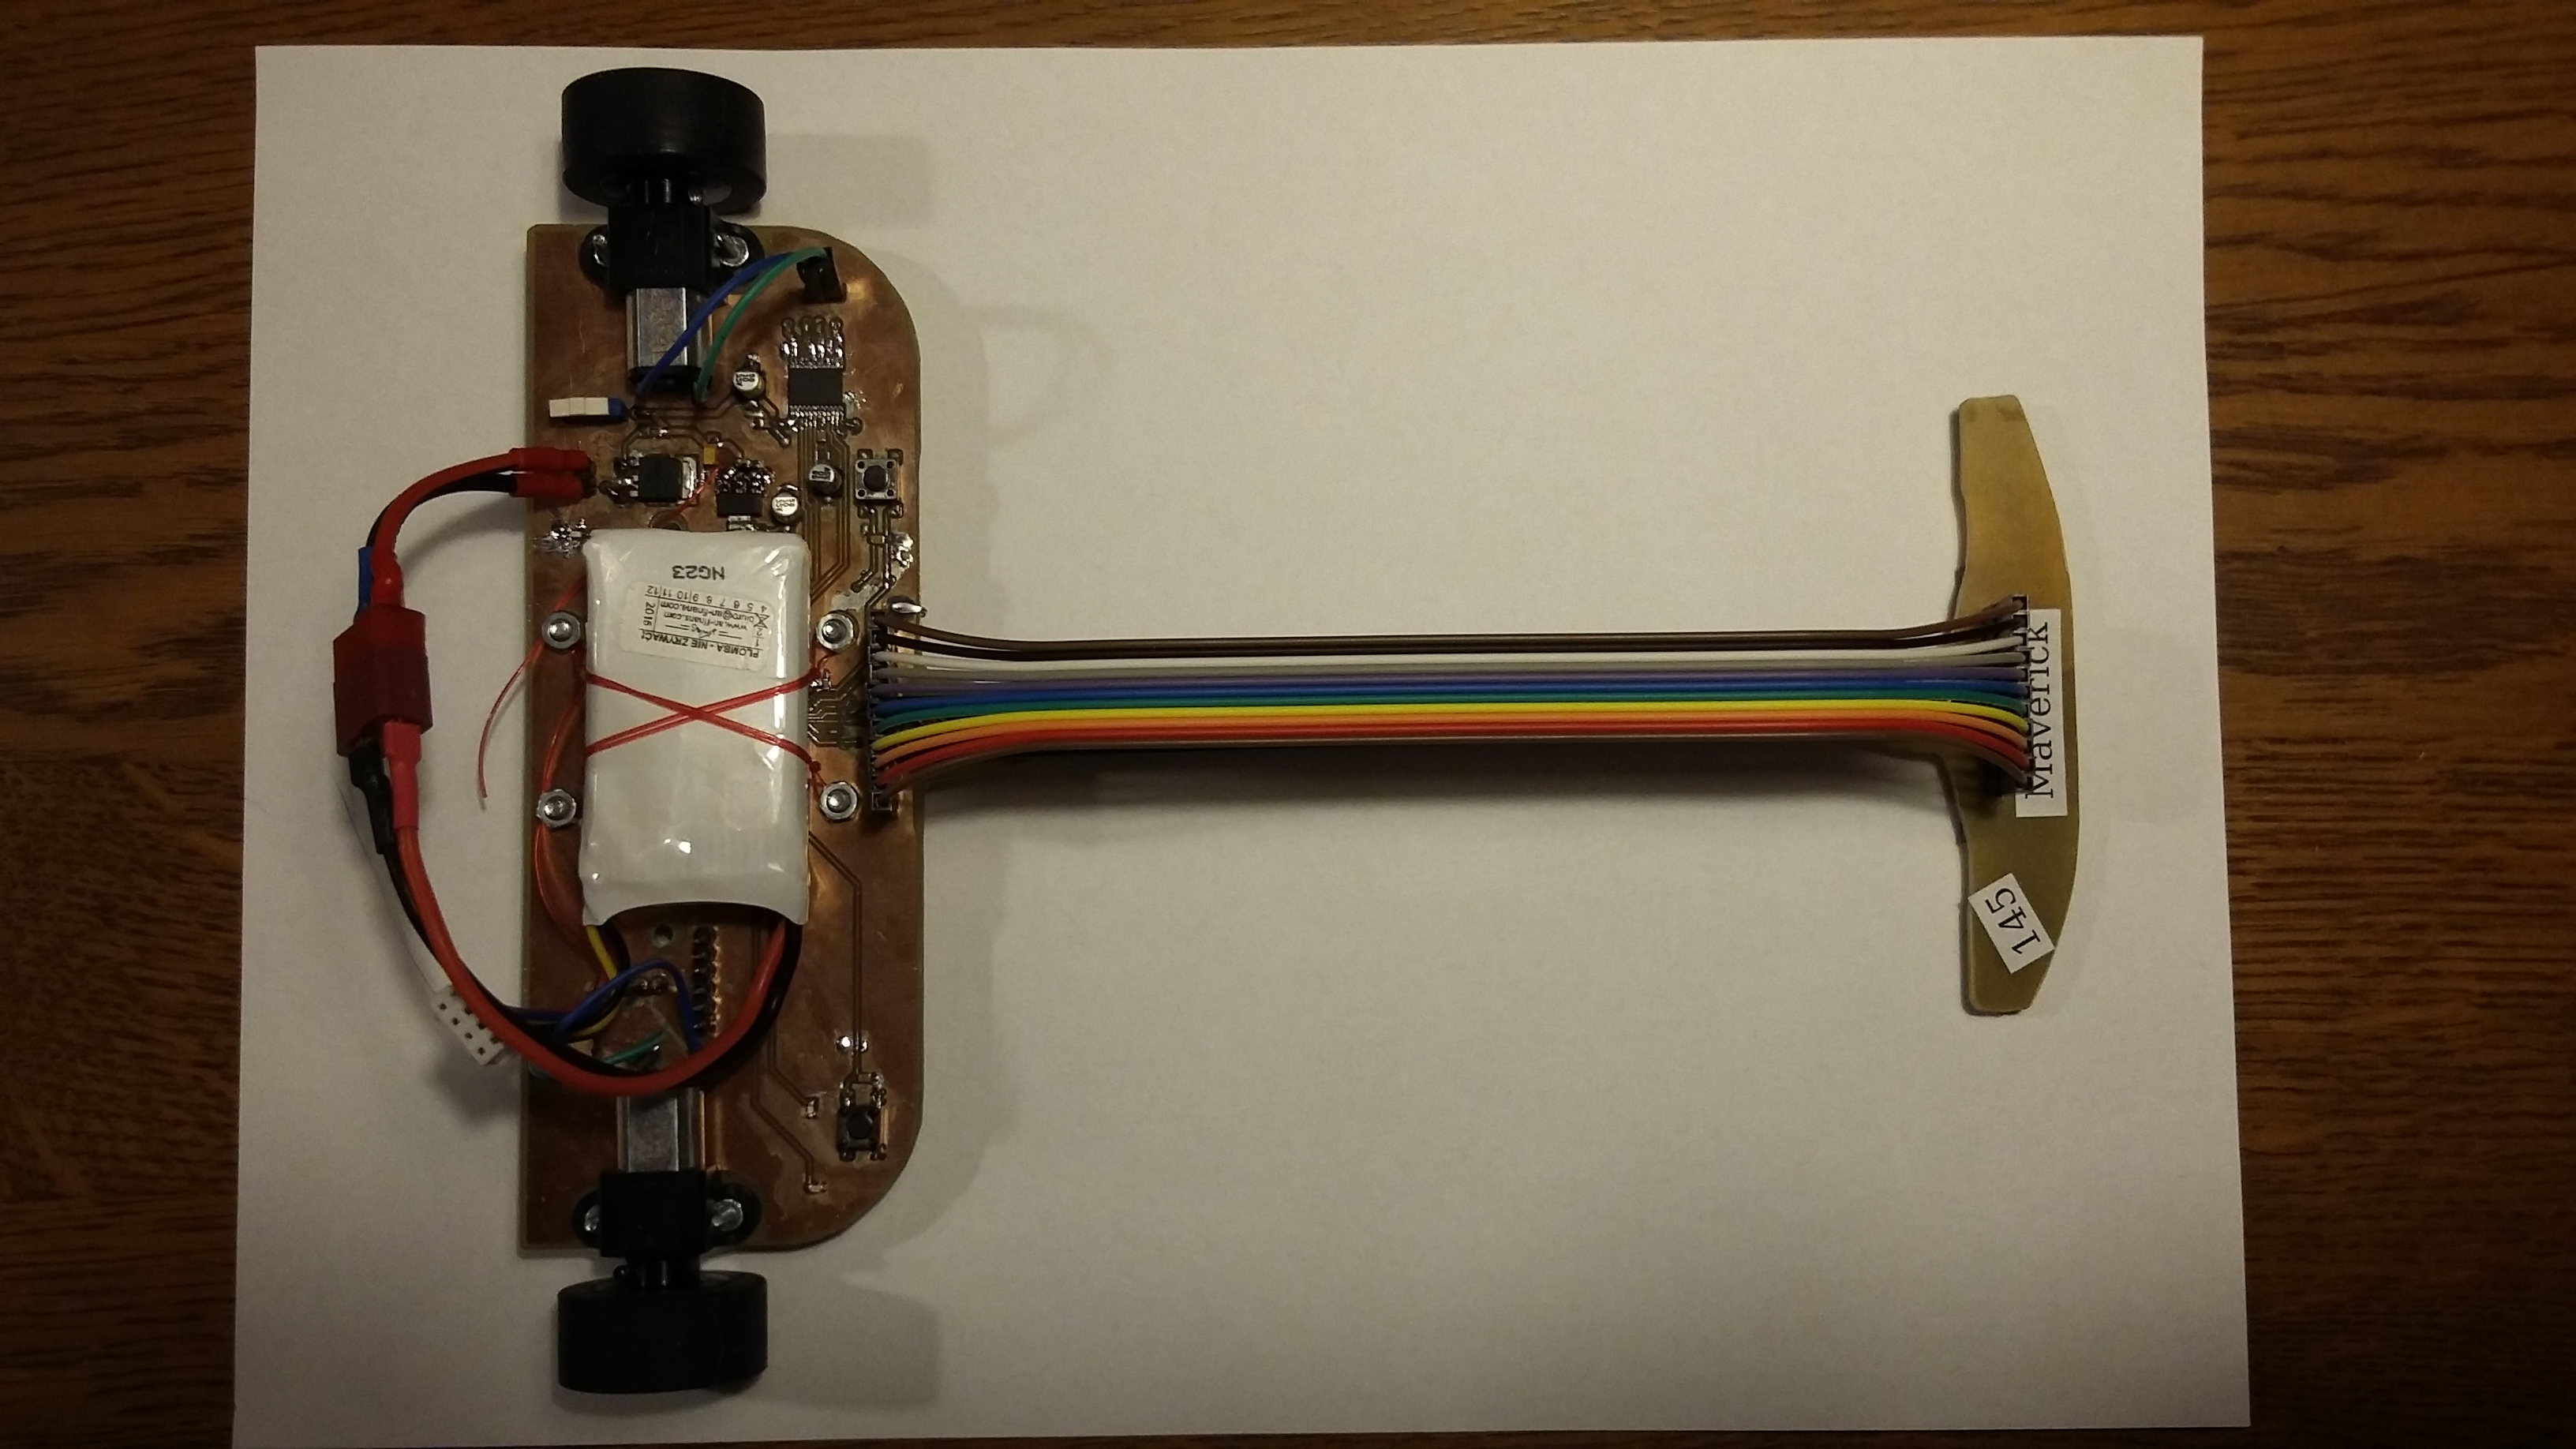
\includegraphics[width=0.4\textwidth]{figures/2.jpg}
    } %Miedzy tymi obrazkami nie ma przerwy, wiec beda zestawione poziomo
    \hspace{0.4cm}
    \subfloat[Tylna płytka\label{subfig:m3}]{%
      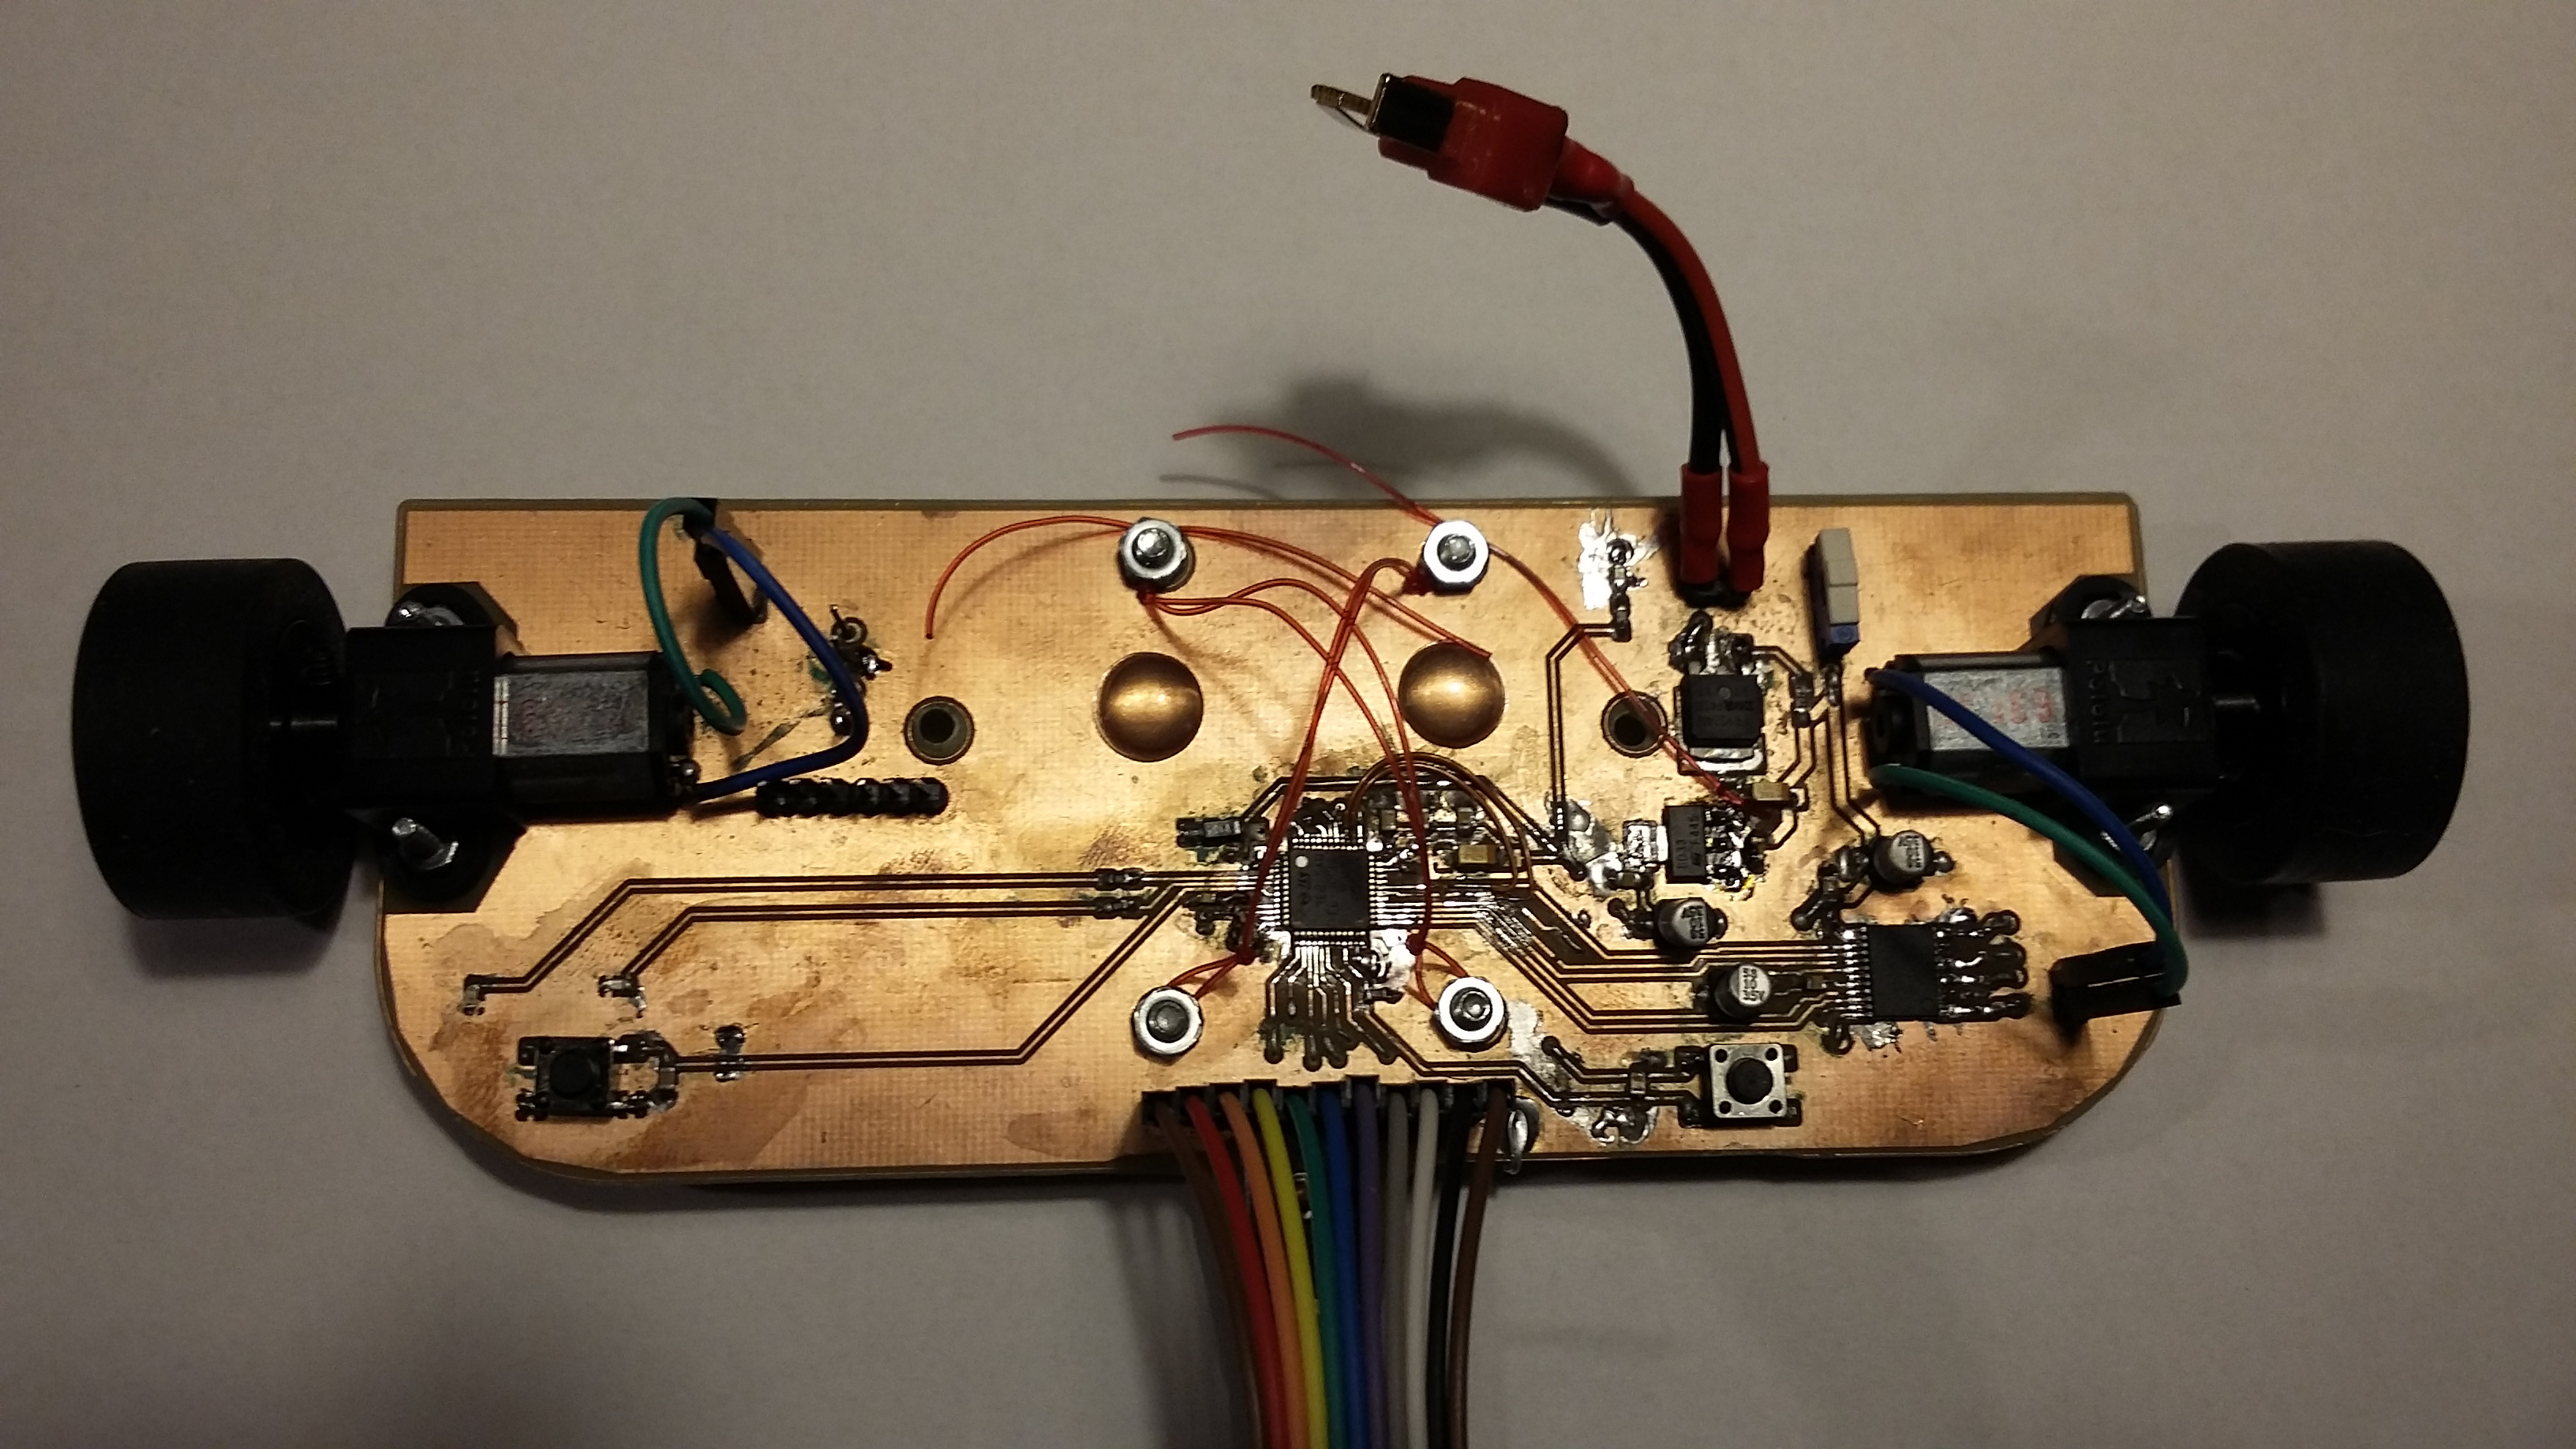
\includegraphics[width=0.4\textwidth]{figures/3.jpg}
    }%Ponizej jest przerwa, wiec nastapi przejscie do nowej linii


    \subfloat[Przednia płytka\label{subfig:m4}]{%
      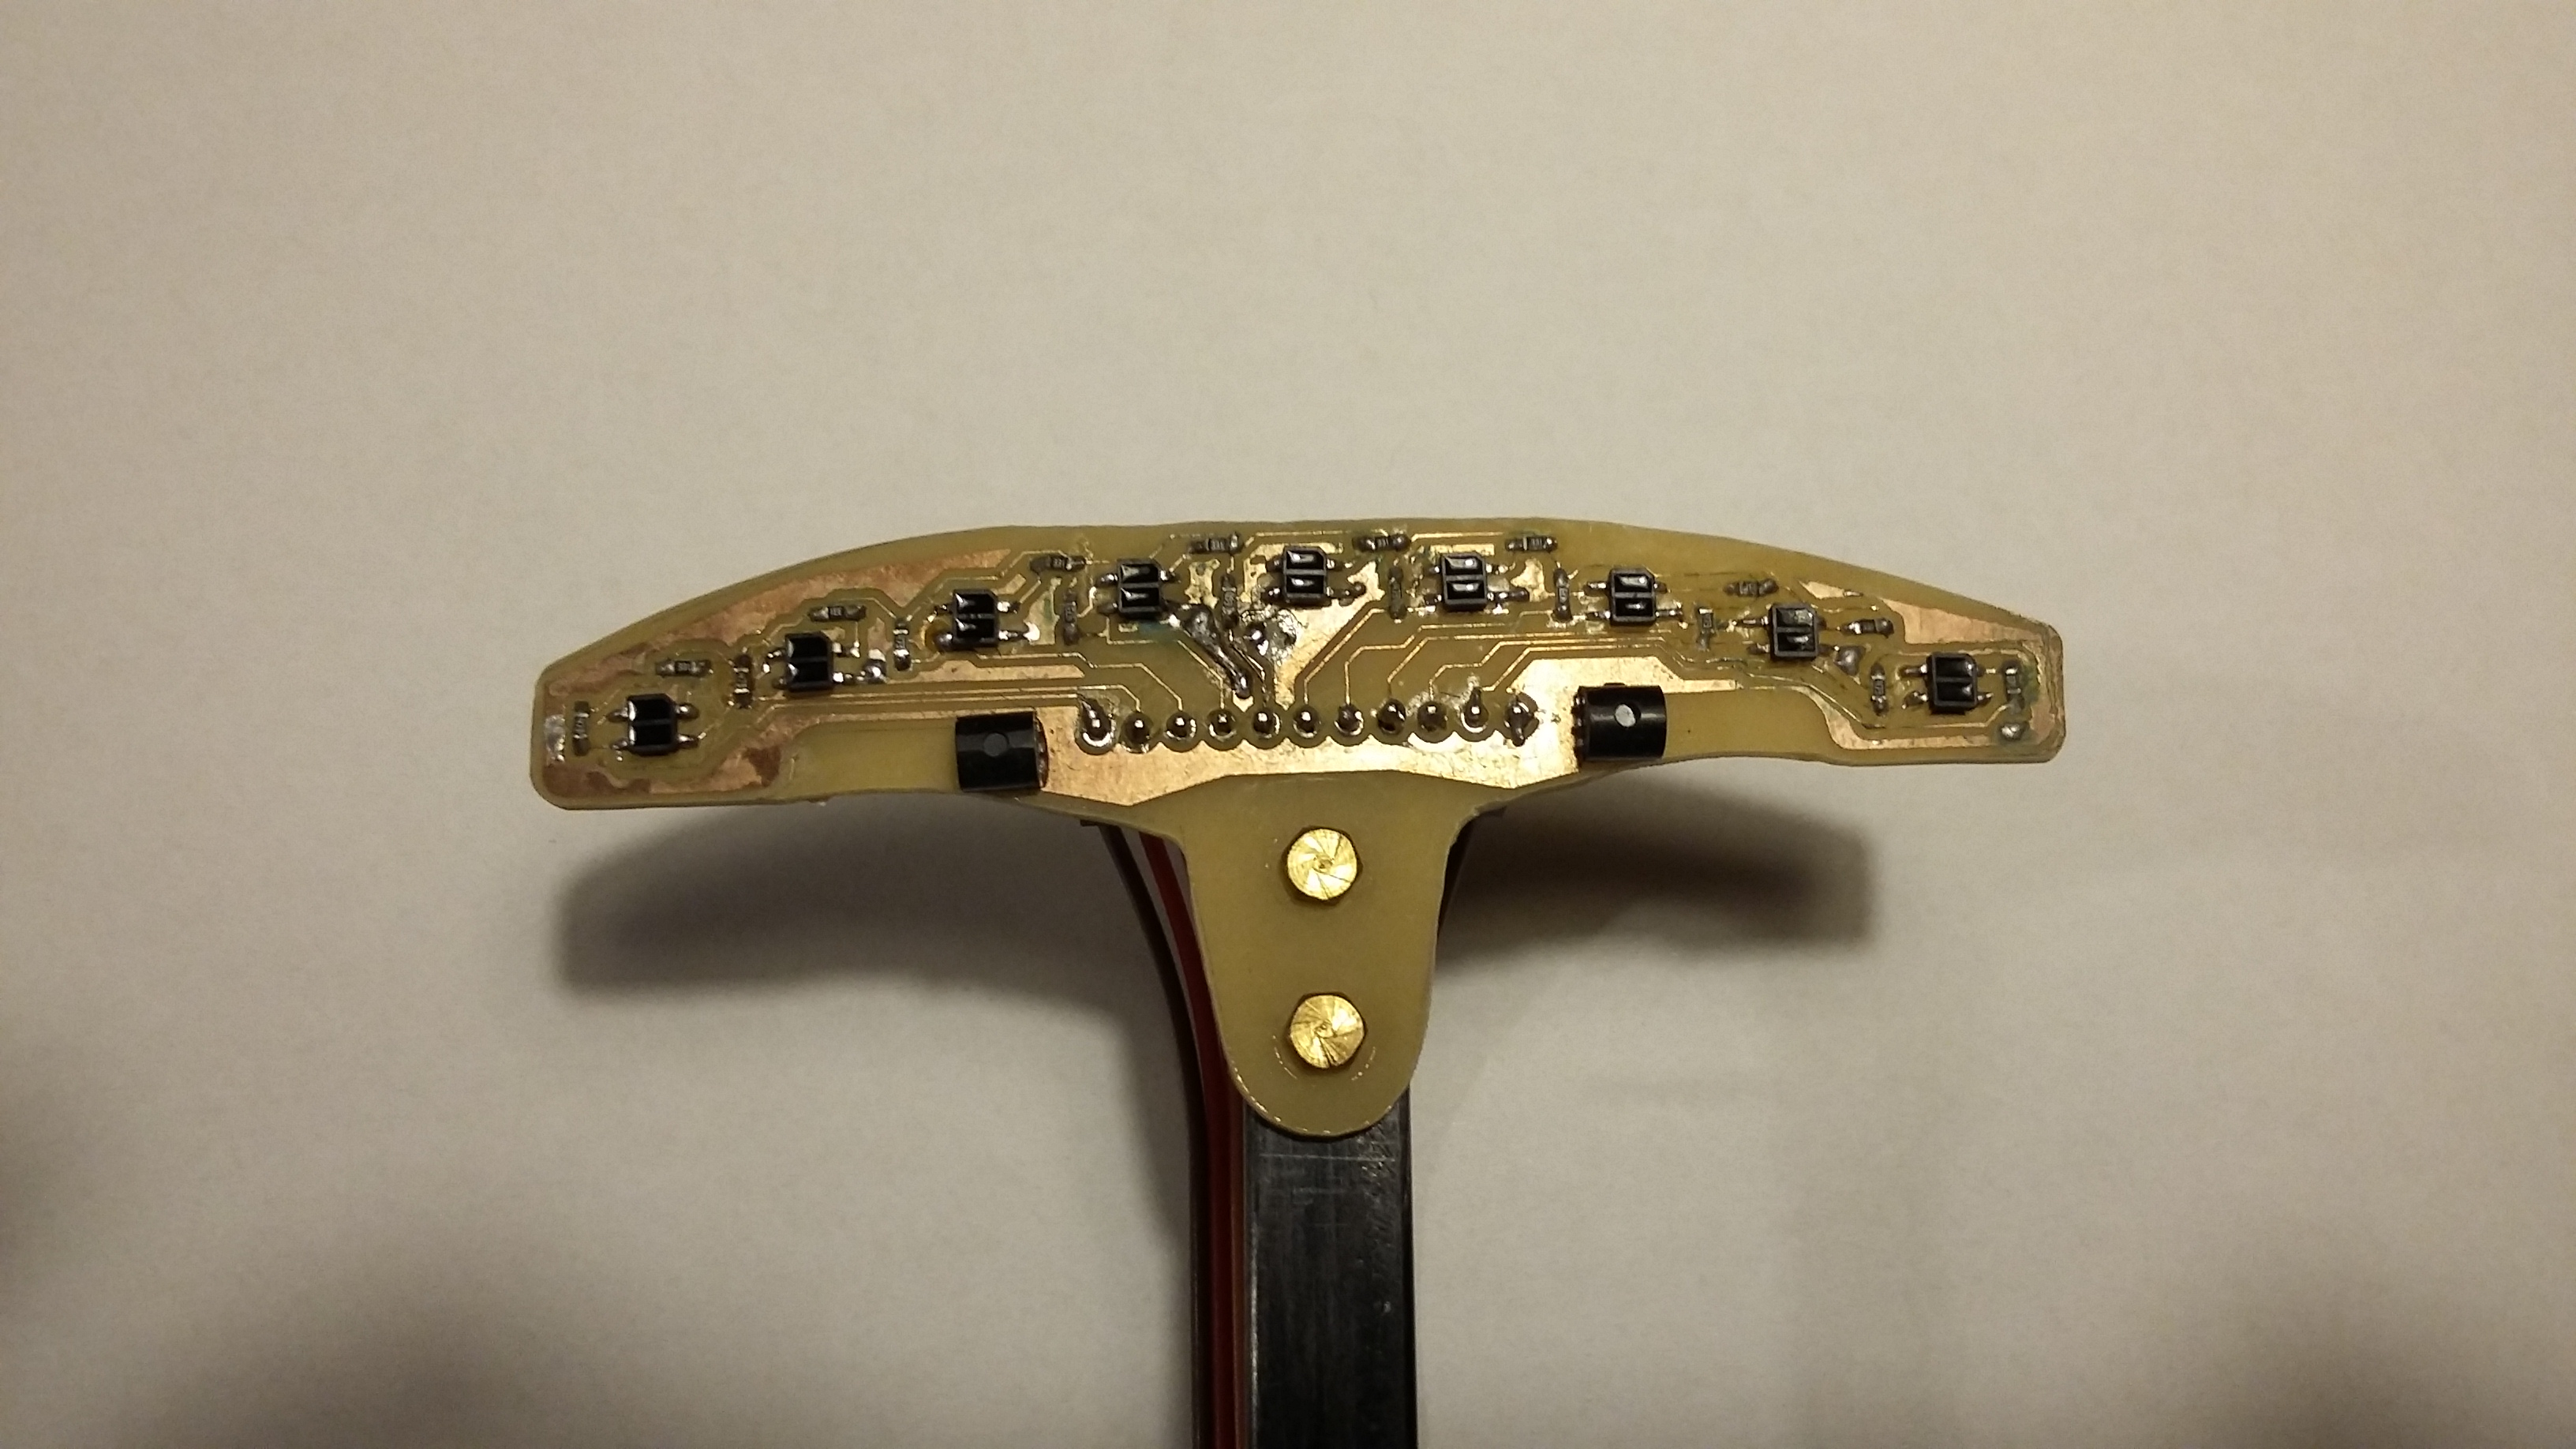
\includegraphics[width=0.4\textwidth]{figures/4.jpg}
    }
    \hspace{0.4cm}
    \subfloat[Widok z boku\label{subfig:m5}]{%
      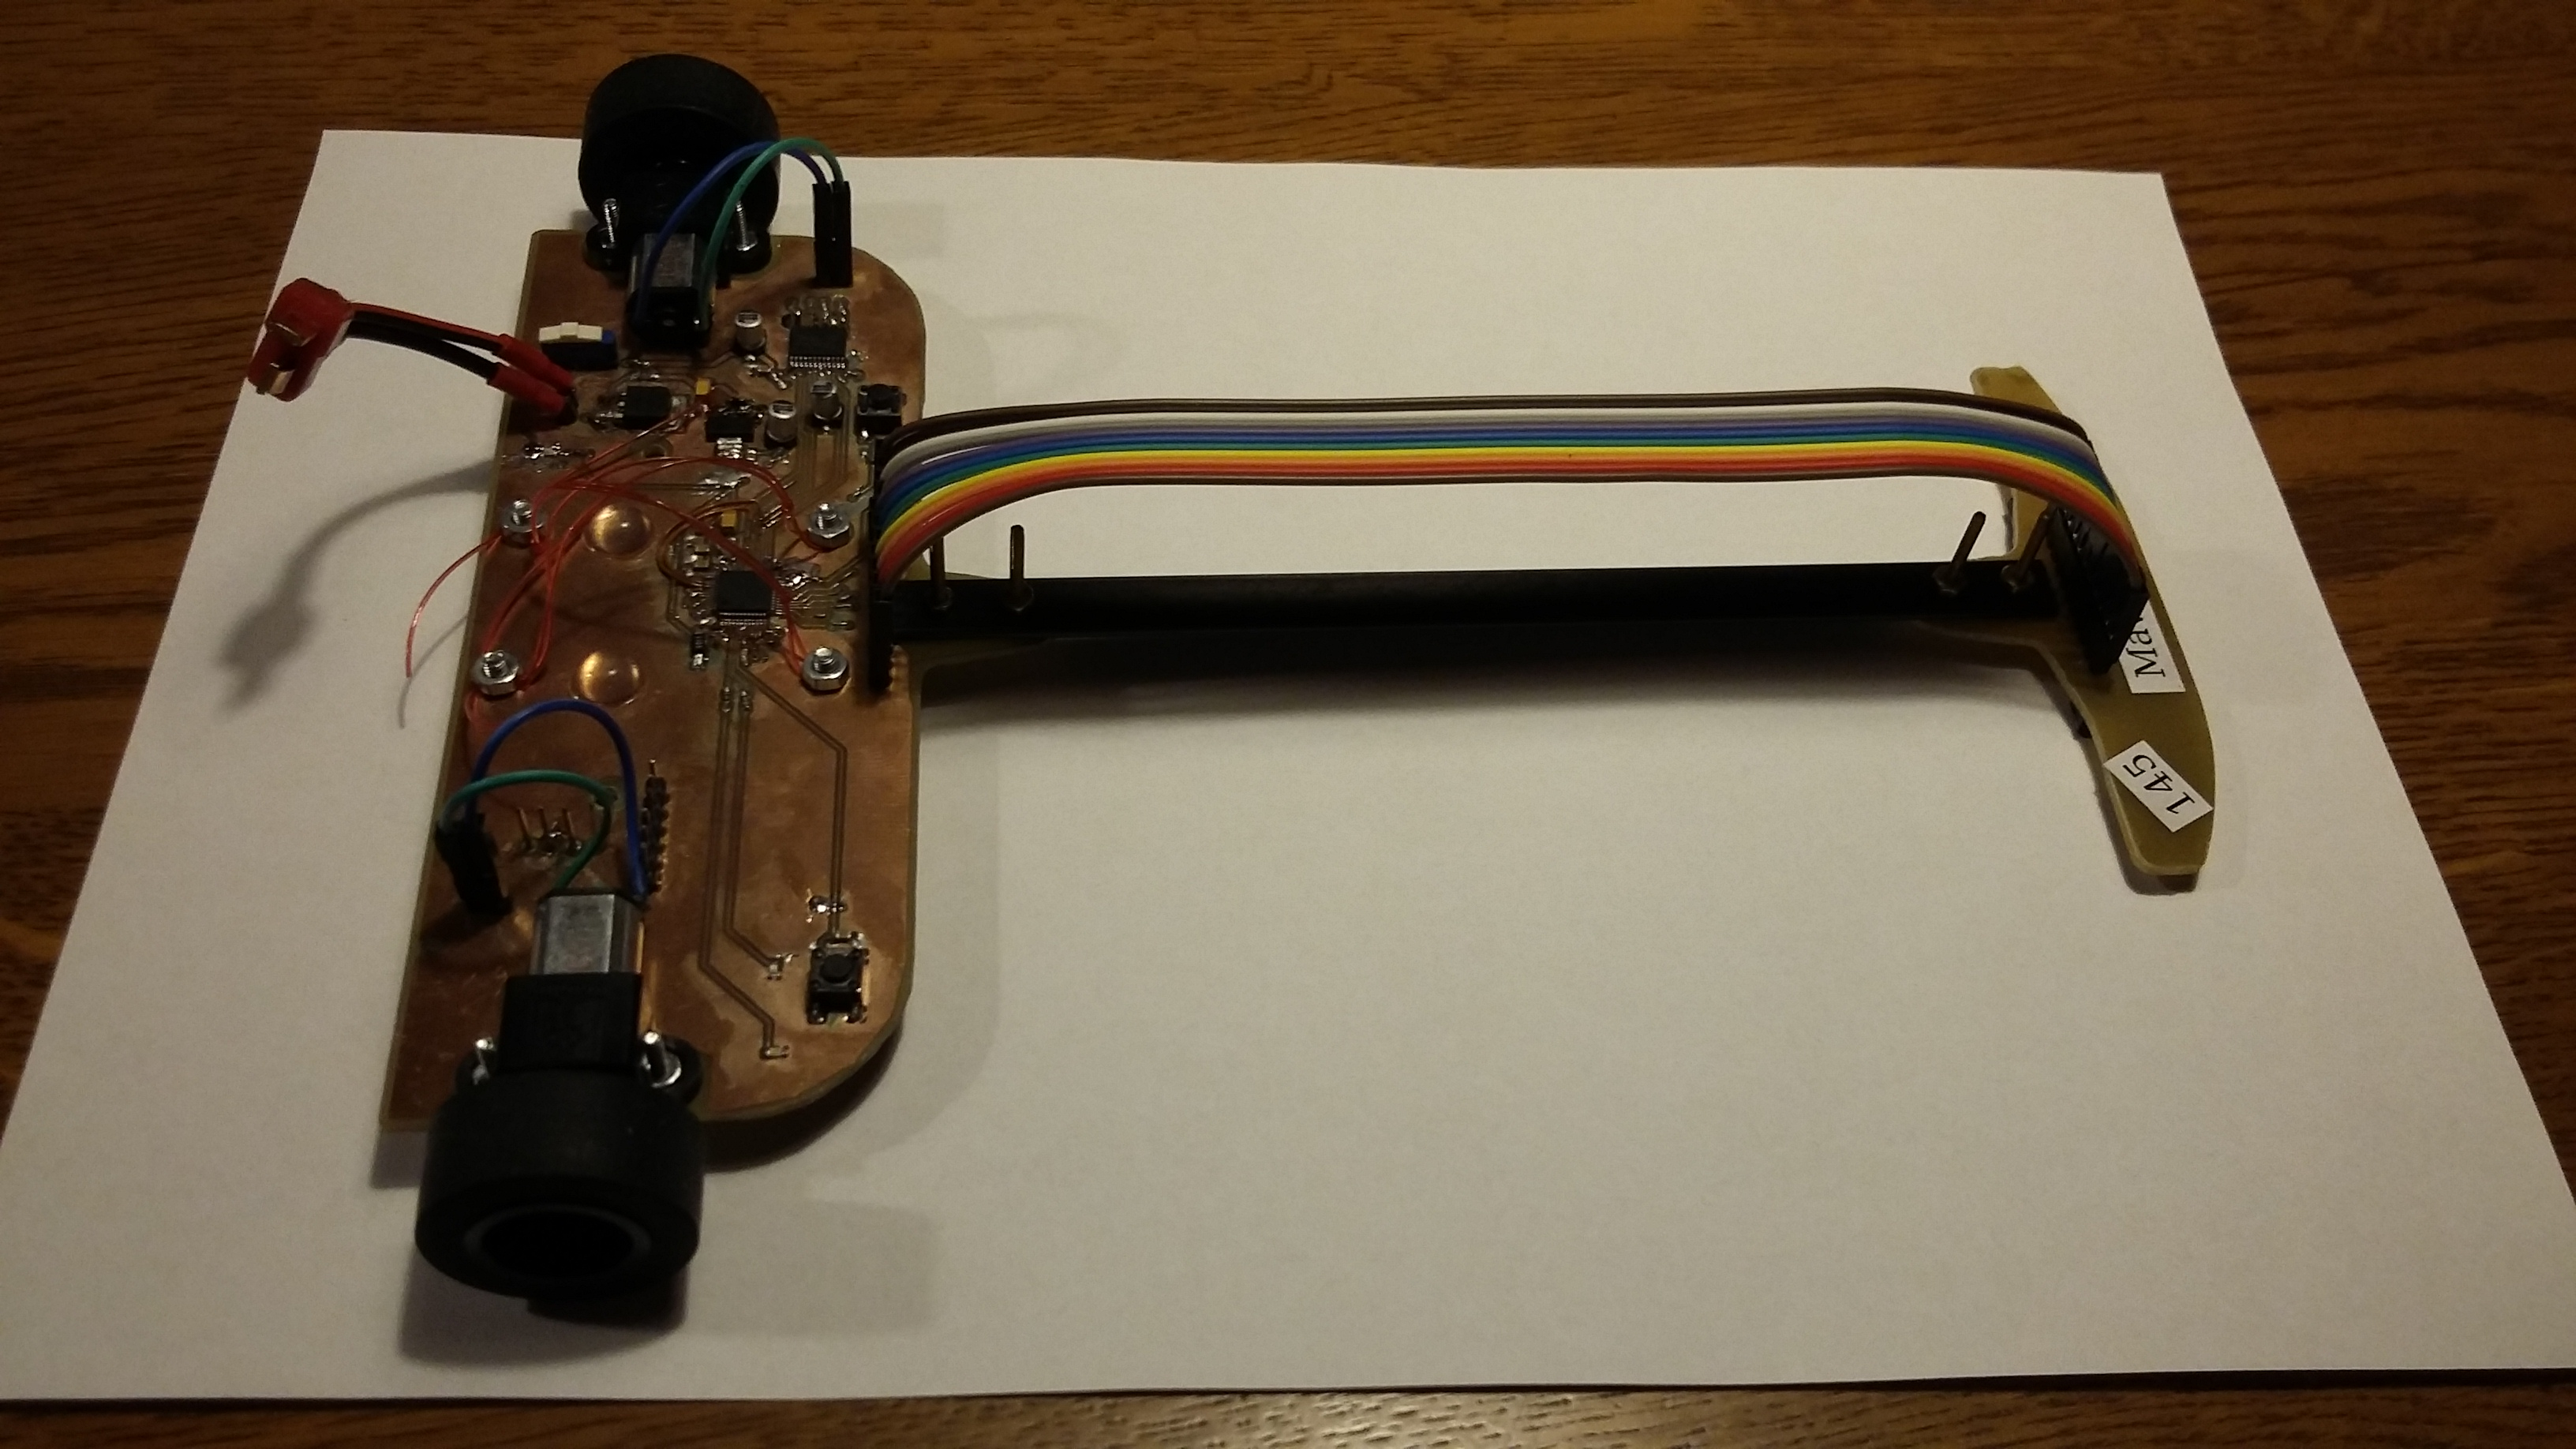
\includegraphics[width=0.4\textwidth]{figures/5.jpg}
    }
    
    \caption{Maverick w różnych ustawieniach}
    \label{fig:maverick}
  \end{figure}%

\begin{figure}[tp]
\centering
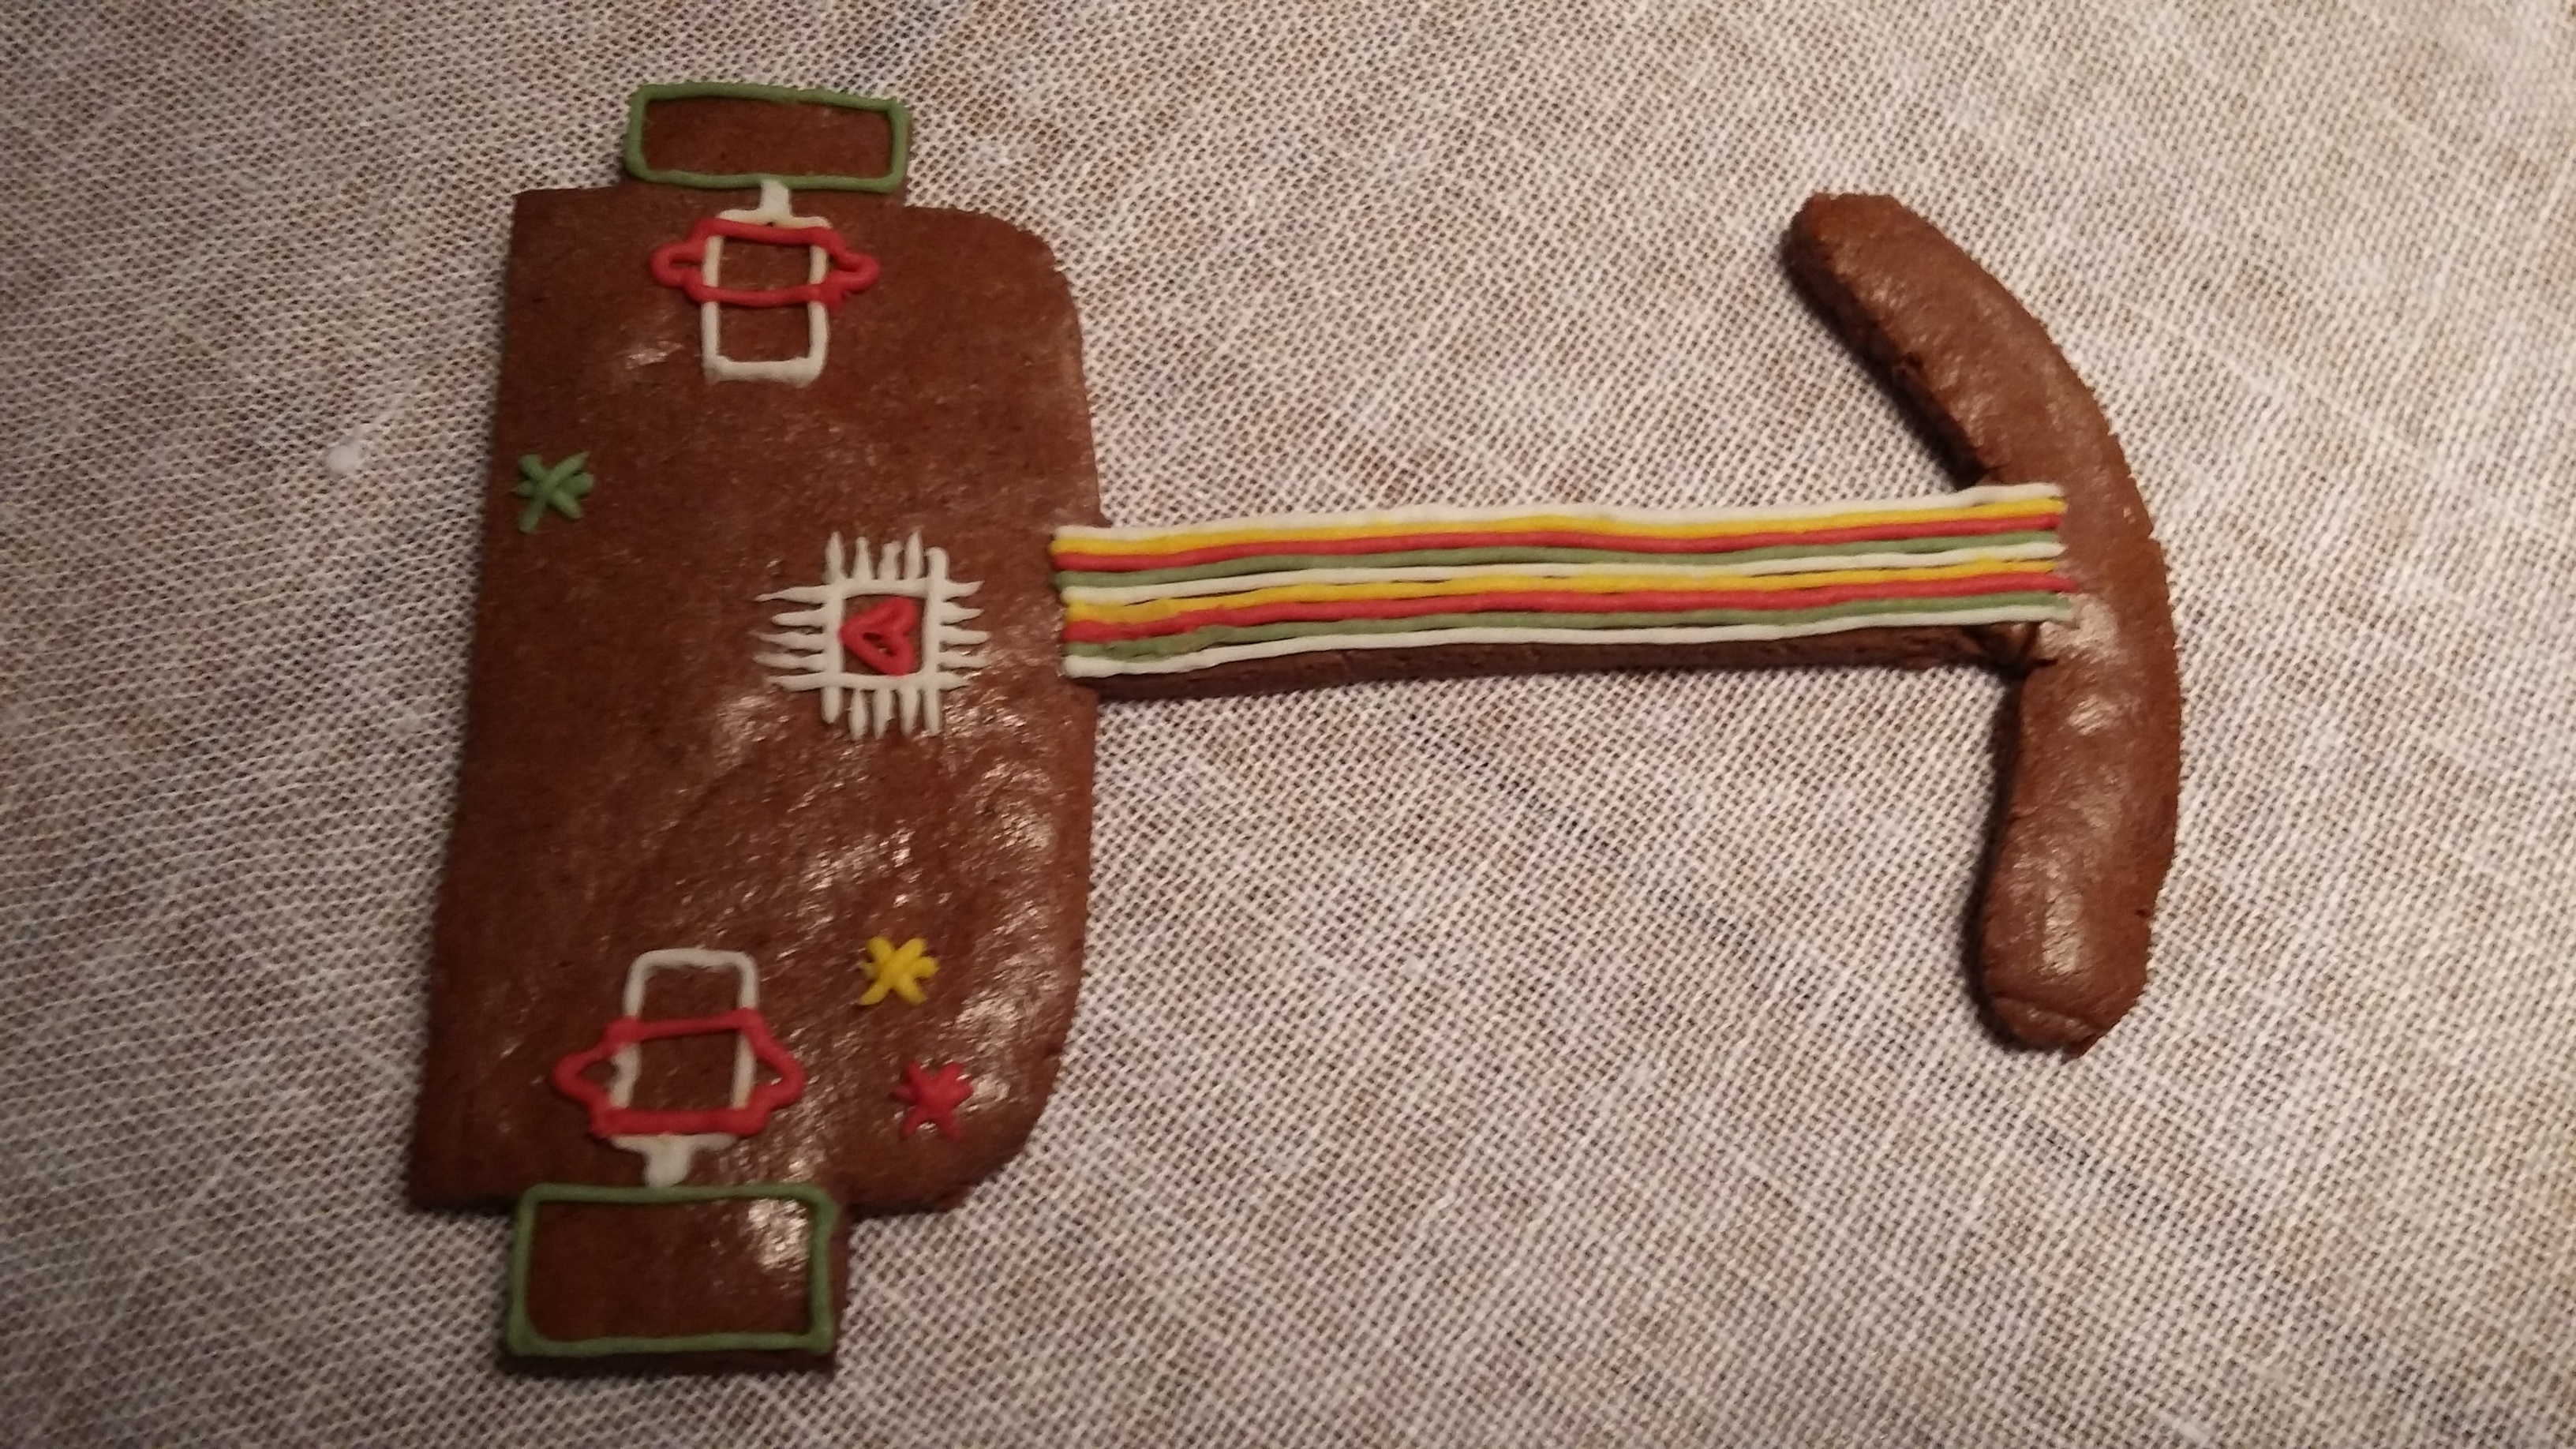
\includegraphics[width=0.9\textwidth]{figures/1.jpg}
\caption{Bonus: Maverick wykonany z piernika \label{fig:p}}
\end{figure}

\end{document}